\documentclass[12pt]{beamer}
\usepackage{polski}
\usepackage[utf8]{inputenc}
\usepackage{graphicx}
\usetheme{Warsaw}
\title{System zautomatyzowanego zarządzania farmą serwerów aplikacji WWW}
\author{Marcin Fabrykowski}
\institute{AGH University of Science and Technology}
\date{17.09.2015}
\begin{document}
\frame{\titlepage}
\begin{frame}
\tableofcontents
\end{frame}

\section{Po co są klastry}

\subsection{Wysoka wydajność}
\begin{frame}
\frametitle{Normalny ruch}
\begin{center}
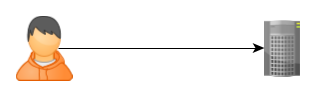
\includegraphics[width=180px]{img/hp1.png}
\end{center}
\end{frame}
\begin{frame}
\frametitle{Większy ruch}
\begin{center}
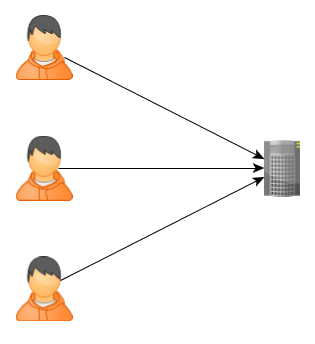
\includegraphics[width=180px]{img/hp2.png}
\end{center}
\end{frame}
\begin{frame}
\frametitle{Jeszcze większy ruch}
\begin{center}
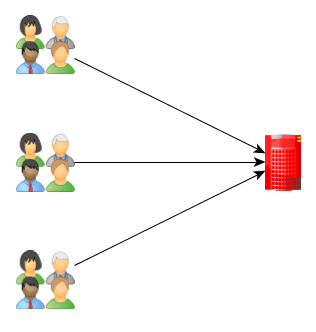
\includegraphics[width=180px]{img/hp3.png}
\end{center}
\end{frame}

\subsection{Wysoka dostępność}
\begin{frame}
\frametitle{Normalna praca}
\begin{center}
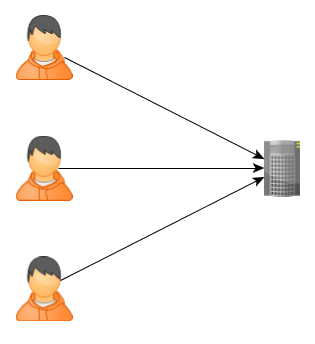
\includegraphics[width=180px]{img/ha1.png}
\end{center}
\end{frame}
\begin{frame}
\frametitle{Awaria serwera}
\begin{center}
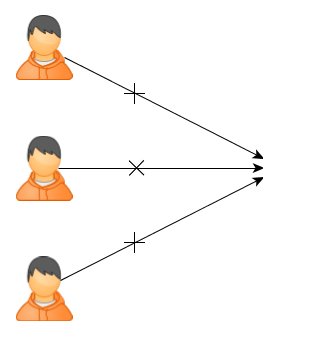
\includegraphics[width=180px]{img/ha2.png}
\end{center}
\end{frame}

\section{Możliwe rozwiązania}
\begin{frame}
\frametitle{Wiele równoległych maszyn}
\begin{center}
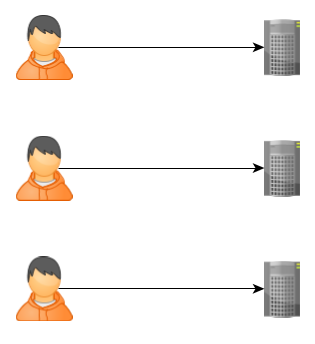
\includegraphics[width=180px]{img/klaster1.png}
\end{center}
\end{frame}
\begin{frame}
\frametitle{Jedna centralna rozdzielająca ruch}
\begin{center}
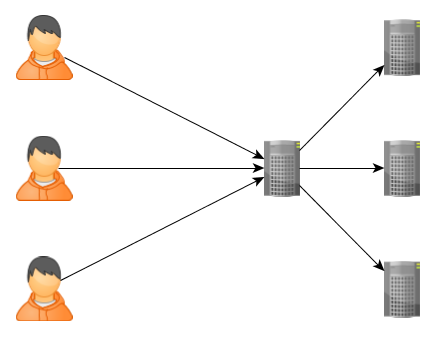
\includegraphics[width=250px]{img/klaster2.png}
\end{center}
\end{frame}

\section{Zarządzanie klasterem}
\begin{frame}
\frametitle{Ręczna konfiguracja}
\begin{center}
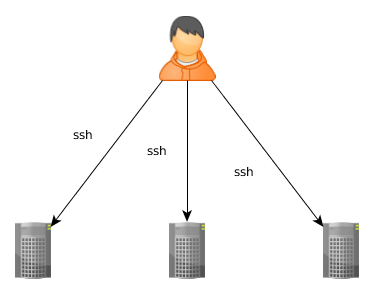
\includegraphics[width=180px]{img/zarzadzanie1.png}
\end{center}
\end{frame}
\begin{frame}
\frametitle{Narzędzie cssh}
\begin{center}
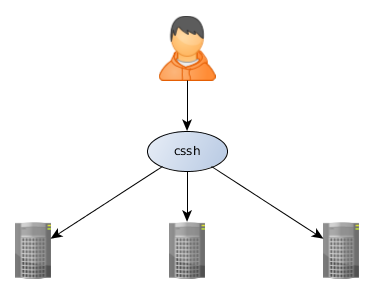
\includegraphics[width=180px]{img/zarzadzanie2.png}
\end{center}
\end{frame}
\begin{frame}
\frametitle{Narzędzie cssh - nowy serwer?}
\begin{center}
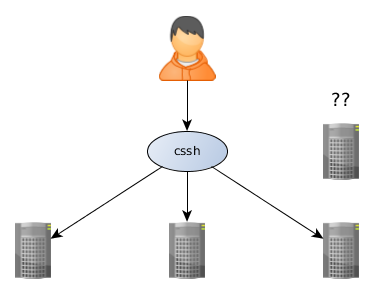
\includegraphics[width=180px]{img/zarzadzanie3.png}
\end{center}
\end{frame}
\begin{frame}
\frametitle{Centralna konfiguracja}
\begin{center}
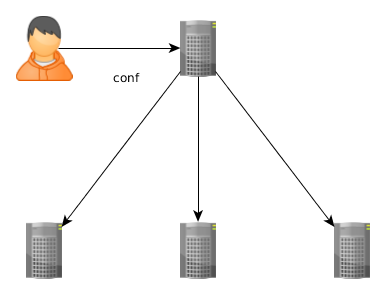
\includegraphics[width=180px]{img/zarzadzanie4.png}
\end{center}
\end{frame}
\begin{frame}
\frametitle{Centralna konfiguracja - nowy serwer?}
\begin{center}
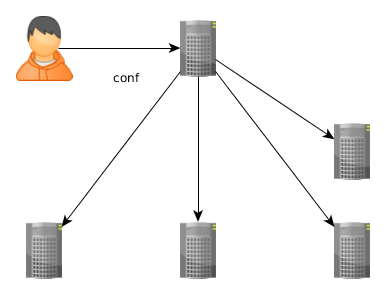
\includegraphics[width=180px]{img/zarzadzanie5.png}
\end{center}
\end{frame}

\section[SZZ]{System zautomatyzowanego zarządzania farmą serwerów aplikacji WWW}
\begin{frame}
\frametitle{System zautomatyzowanego zarządzania farmą serwerów aplikacji WWW}
\begin{center}
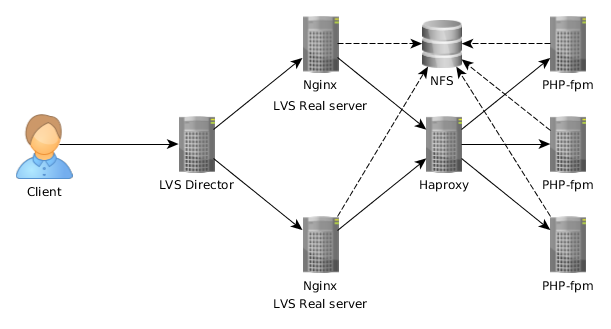
\includegraphics[width=250px]{img/struktura_szz.png}
\end{center}
\end{frame}
\begin{frame}
\frametitle{System zautomatyzowanego zarządzania farmą serwerów aplikacji WWW}
\uncover<1->{
Co może SZZ:
\begin{itemize}
\item skonfigurować klaster WWW
\item czuwać, aby nie konfiguracja nie zmieniała się
\item w prosty sposób dodawać nowe węzły do klastra
\end{itemize}
}
\uncover<2->{
Czego nie może SZZ:
\begin{itemize}
\item w pełni zastąpić administratora
\end{itemize}
}
\end{frame}
\frame{\titlepage}

\end{document}
